\section{Research Plan and Methodology} \label{sec:rep}

This section takes a thorough approach to tackle concurrency attacks, including 
its program analysis model, a novel detection approach to detection such 
attacks via leveraging this model, and a runtime infrastructure to defense 
attacks.

\subsection{Modeling Concurrency Attacks} \label{sec:model}

% P1: as mentioned in background, a key reason is thread interleavings, 
% so we need to reason about the general patterns we have. Or we say our 
% methodology is just like pattern matching.
As mentioned in \S\ref{sec:background}, state-of-the-art lacks a rigorous model 
for concurrency attacks. Specifically, people lack understanding on how 
concurrency bugs propogate to security-sensitive operations in source code, and 
how we can use program analysis approaches to describe this propogation. This 
section first gives two concrete examples on concurrency attacks 
(\S\ref{sec:}), and then propose our model.

\subsubsection{Concurrency Attacks Examples} \label{sec:examples}

\begin{figure}[t]
\centering
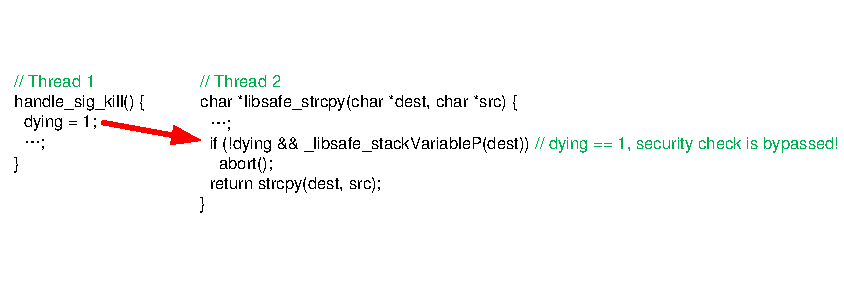
\includegraphics[width=0.99\columnwidth]{figures/libsafe}
\vspace{-.05in}
\caption{{A concurrency attack in libsafe.}} \label{fig:libsafe}
\vspace{-.05in}
\end{figure}

Figure~\ref{fig:libsafe} shows the simplified code of a concurrency attack in 
\libsafe, a popular stack overflow protection library. In short, this library 
provides its own safe memory and string operations functions. In this 
functions and carefully checks whether a stack variable is passed in as 
function arguments and whether this function may overflow the call stack. If a 
program is dying, such checks are disabled. Unfortunately, a global varible 
\v{dying} is not protected by mutex locks, so attackers can leverage two 
threads to trigger a data race bug on this variable, bypass the security 
check, overflow the function's return address of the stack, and then makes the 
program execute malicious code from inputs. Ironically, this \libsafe library 
is no longer ``safe" in the mulithreading era.

\begin{figure}[t]
\centering
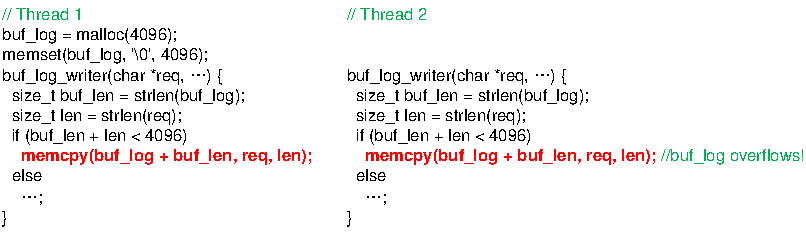
\includegraphics[width=0.99\columnwidth]{figures/apache}
\vspace{-.05in}
\caption{{A concurrency attack in Apache.}} \label{fig:apache}
\vspace{-.05in}
\end{figure}

Figure~\ref{fig:libsafe} shows the simplified code of a concurrency attack in 
\apache, a widely used web server to manage http pages from different users. 
\apache spawns a number of threads, with each to server a httpd request. Each 
thread logs each http request it receives into a global log buffer and flush 
this buffer to a log file when the log is full. However, developers missed a 
mutex lock to protect this buffer, so this buffer can overflow and corrupt 
other memory in heap. Unfortunately, \apache puts the log file's descriptor next 
to this log buffer. If this descriptor is corrupted, \apache may write the 
request log to arbitrary files. Our riliminary study have successfully corrupted 
this file descriptor and writes the request logs to http pages owned by regular 
users, violatinng integrity of \apache.

\subsubsection{Concurrency Attacks Program Analysis Models} 
\label{sec:attack-phase}

% P3: pattern.
These two examples appear to be diverse, but they have a few common elements in 
order to construct a concurrency attack. First, corrupted global memory is 
necessary (\eg, \v{dying} in \libsafe, and the \v{buf\_len} in \apache). 
Second, a security-sensitive operation is necessary (\eg, \v{strcpy} and 
\v{memcpy}). Third, the courrupted global memory must cause abnormal behavior of 
the security-sensitive operation. For example, the abnormal behavior in \libsafe 
is we must leverage the corrupted memory to bypass the security check. For 
\apache, we leverage the corrupted memory to bypass the security check. In this 
case, the corrupted memory may just have indirect impact on the 
security-sensitive operation (\ie, its corrupted value does not flow to the 
operation), or have direct impact (\ie, the corrupted memory, buffer log, is 
part of the operation).

In sum, three key elements compose a concurrency attack: corrupted memory, 
security-sensitive operation, and impact (indirect or direct) from the memory 
to the operation. In the PL community, we cause the indirect impact as control 
dependency, and the direct impact data dependency. Actually, not only for these 
examples, the \nattacks attacks we have reproduced and the \noldattacks in 
previous study~\cite{con:hotpar12}, they all have these three key elements.

% PX: emphasis the contribution/potential value of this model.
In a high level, this model treats a concurrency attack as a source-sink model, 
where a source is a courrupted global memory caused by a concurrency bug, and a 
sink is a security-sensitive operation. Then this model tracks the data flow 
and control flow of the corrupted memory to the sensitive operations. Unlike a 
traditional model which only consider inputs as the source, our model considers
concurrency bugs as the the inputs. This model spurs several interesting 
research questions. First, how do we track down the corrupted memory in the 
middle of an execution? Second, given that concurrency bugs are not only just 
one, how does our analysis handle multiple concurrency bugs (\eg, multiple 
corrupted variables)? Third, given that not all security-sensitive operations 
are indeed relevant to the source, how do we prune the irrelevant operations 
soundly (\ie, without missing exploits)? In \S\ref{sec:detect}, we plan to 
leverage this model to develop an effective detection approach, and our 
priliminary work has shown promissing results on addressing these research 
questions.

% TBD: add a table on the list of concurrency bugs and the list of dangerous 
% operations.



% P5: how to handle unknow patterns? Just say patterns in our work may spur new 
% patterns. We will continue to find new patterns as well.
% P5: TBD.

% \subsubsection{Concurrency Attacks with Three Common Patterns}
% \label{sec:model-pattern}

% Goal 1: modeling.

\subsection{Detecting Concurrency Attacks in Testing Phase}\label{sec:detect}

TBD.

\begin{figure}[t]
\centering
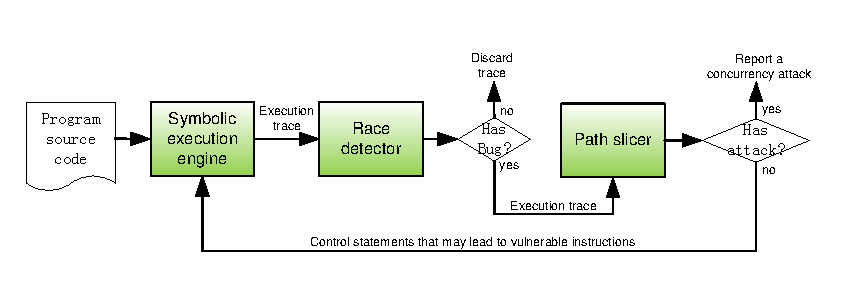
\includegraphics[width=0.5\columnwidth]{figures/detection}
\vspace{-.05in}
\caption{{Workflow of the concurrency attack detection scheme.}} 
\label{fig:detection}
\vspace{-.05in}
\end{figure}

\subsubsection{Workflow of \xxx's Detection Scheme}\label{sec:detect-arch}

% P1: why need a detection scheme. First, capture as many as exploits in 
% testing phase. And call for re-install if there is any potential exploit. Even for 
% old concurrency bugs, it is still necessary because exploits may have already 
% occured and attackers may have already broken in.

% P2: two research questions. Given a concurrency bug, will it lead to an 
% exploit?

% P3: if this bug may lead to an exploit, what inputs may lead to such exploits?

% P4: how to incorporate the patterns in previous section?

% P5: go over the workflow, which is a straight line of boxes. May add some 
% back edges to make it an iterative approach?
 
% \subsubsection{Implementing \xxx's Detection Scheme}\label{sec:detect-impl}
% TBD

\subsubsection{Priliminary work}\label{sec:detect-result}

% P1: we have implemented part of the dangerous operation. pointer NULL 
% derefence. Report the results. FP:FN.

\subsection{Defensing Concurrency Attacks in Deployment Phase} 
\label{sec:defense}

% P1: motivation, why runtime detection is important. We want to mostly avoid 
% exploits by preventing attackers from manipulating the schedules.
Although \S\ref{sec:detect} has proposed an detection scheme for developers to 
find concurrency attacks in the testing phase, this scheme can not catch 100\% 
attacks because it is designed to find attacks on the concurrency bugs it meets 
at runtime. Thus, to practically prevent concurrency attacks taking over 
multi-threaded programs in the deployment phase, an efficient, transparent 
runtime infrastructure is needed to defense concurrency attacks.

% P2: reason 2: when races occur even if Parrot is enforced, we want to have 
% fault-tolerance.
To build a defense infrastructure, I propose to leverage state machine 
replication (or \smr), a powerful fault-tolerance concept in today's 
distributed system and clouds. \smr models a program as a deterministic
state machine, where the states are important program data and the transitions 
are deterministic executions of program code under input requests. SMR runs 
replicas of the program and invokes a distributed consensus protocol 
(typically \paxos) to ensure the same sequence of input requests for replicas, 
as long as a quorum (typically a majority) of the replicas agrees on the input 
request sequence. Under the deterministic execution assumption, this quorum of 
replicas must reach the same exact state despite various exceptions such as 
program failures or network partitions. SMR is proven safe in theory and 
provides high availability in practice.

The fault-tolerant benefit of \smr makes it particularly attractive
on implementing a principled replication system for tolerating concurrency 
attacks. Unfortunately, doing so is quite challenging, and I forsee four 
challenges.

% P3: reason 3: we want survive. checkpoint and re-execute, and diversify the 
% schedules before re-execute. Sell it like a self-healing runtime system.
First, today’s multithreaded programs are almost universally
multithreaded, thus even concurrency attacks do not manifest, the programs 
running across replicas can still easily run into different thread schedules 
and divergent execution states. Second, to leverage existing SMR systems such 
as ZooKeeper, developers often have to shoehorn their programs into the 
narrowly defined state machine interfaces provided by these SMR systems. Third, 
such a runtime infrasture should run almost as fast as the native executions in 
the deployment phase. Fourth, if replicas run into buggy schedules that trigger 
concurrency attacks, our infrastructure should be able to recover from the 
attacks.

\subsubsection{Architecture of \xxx's Runtime Defense Infrastructure} 
\label{sec:defense-arch}

\begin{figure}[t]
\centering
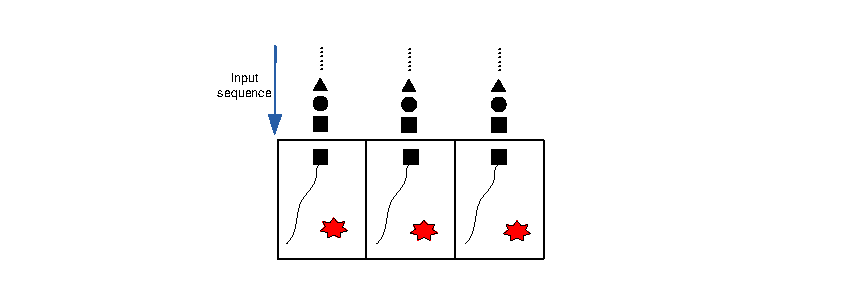
\includegraphics[width=0.3\columnwidth]{figures/defense}
\vspace{-.05in}
\caption{{A runtime infrastructure to defense concurrency attacks.}} 
\label{fig:defense}
\vspace{-.05in}
\end{figure}

To address these challenges, I propose a \smr-based replication 
system. With this infrastructure, a developer focuses on implementing her 
program’s intended functionality, not how to defense concurrency attacks. When 
she is ready to replicate her program for strengthened security, she simply
runs this infrastructure with her program on multiple replicas. Within
each replica, this infrastructure interposes on the socket and the thread
synchronization interfaces to keep replicas in sync. Specifically, to address 
the first challenge, it considers each incoming socket call (e.g., accept() a 
client’s connection or recv() a client’s data) an input request, and runs a 
\paxos consensus protocol to ensure that a quorum of the replicas sees the same 
exact sequence of the incoming socket calls.

To address the second challenge, this infrastructure schedules synchronizations 
using deterministic multithreading (DMT). This technique
typically maintains a logical time2 that advances deterministically on each 
thread's synchronization. By serializing thread synchronizations, DMT 
practically makes an entire multithreaded execution deterministic. The overhead
of DMT is typically moderate because most code is not synchronization and can 
still run in parallel.

\begin{figure}[t]
\centering
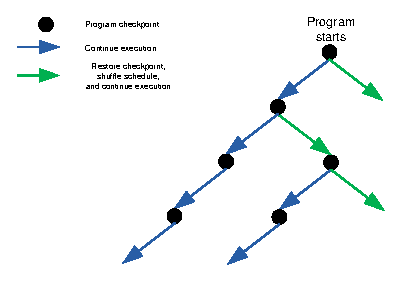
\includegraphics[width=0.3\columnwidth]{figures/healing}
\vspace{-.05in}
\caption{{The self-healing idea for recovering from concurrency attacks.}} 
\label{fig:healing}
\vspace{-.05in}
\end{figure}

% Mention the self healing idea.
To address the fourth challenge, we propose a self-healing idea 
(Figure~\ref{fig:healing}), which leverage existing transparent program 
checkpoint and restore techniques. On program starts, one backup replica first 
checkpoints the program, and then the program runs as is. Once minor replicas 
hit concurrency attacks, the other replicas can still agree on new inputs and 
process requests. If all replicas fail due to hitting the same vulnerable 
schedule, we simply extracts a previous checkpoint, shuffle the schedules, and 
then let the program continues to execute. To this end, this idea checkpoint 
and recovery must work with general programs with its file system. To this end, 
it leverages CRIU to checkpoint and restore process states, and LXC for file 
system states.

As a typical security setting, we need to define which components of 
this Infrastructure must be trusted. In this project, we require the 
infrastructure and the checkpoints are trusted (\ie, even if the program 
compromises, its program checkpoints and the infrastructure are not effected). 
We consider this requirement as reasonable, because once this infrastructure is 
built, we can leverage existing verification techniques to focus on verifying 
this infrastructure, and on top of it, we no longer need to verify those 
programs.




% P4: challenges on doing so. Including the initial work.

\subsubsection{Priliminary work} \label{sec:defense-result}

% P1: we have built a replication system. Perf and checkpoint results.
My collaborators and I have built a propotype system~\cite{crane:sosp15} to 
address the first two challenges. \crane has shown to be able to transparently 
and efficiently support four general multithreaded programs without modifying 
them. We have also shown that this infrastructure is robust on primary replica 
or backup failures. For the third challenge, we plan to study more 
programs and see whether we can leverage performance hints to optimize 
performance. For the fourth challenge, our propotype system \crane has 
implemented a basic checkpoint/restore feature.

\subsection{Research Plan} \label{sec:rep}
time line. R1 R2.


